\documentclass[a4paper]{article}

\usepackage[utf8]{inputenc}
\usepackage[T1]{fontenc,url}
\usepackage{cite}
\usepackage{hyperref}
\usepackage{amsmath, amssymb}
\usepackage{tikz}
\usepackage{graphicx}
\usepackage{parskip}
\usepackage{lmodern}
\usepackage{algorithm}
\usepackage{algpseudocode}
\usepackage{epigraph}
\usepackage{listings}
\usepackage{float}
\usepackage{amsthm}
\usepackage{changepage}
\usepackage{listings}



\begin{document}
\title{FYS4150 -- Project 3}
\author{Joachim Falck Brodin,
        Fredrik Jaibeer Mahal Nordeng,\\ 
        and Endrias Getachew Asgedom}

\maketitle
\begin{abstract}
\noindent
\end{abstract}
Two numerical algorithms, the Forward Euler and the Velocity Verlet, are used for solving the $n$-body problem of the solar system dynamics. The resulting system of coupled ordinary differential equations are discretized and transformed into an initial value problem. The performance of the two algorithms is tested using the simple two-body problem consisting of the Earth and the Sun. The Velocity Verlet algorithm outperforms the Forward Euler in terms of accuracy, stability, and conservation of energy and angular momentum. We expect the Forward Euler algorithm to be faster than the Velocity Verlet, as it contains less floating point operations, but for the simple two-body problem the two algorithm's time consumption is equivalent. Using the Velocity Verlet algorithm, we show that the Earth follows a stable elliptical trajectory around the Sun, only when the gravitational force is an inverse square law. Combining our simulation of the two-body problem with the bisection method, we determine the escape velocity of the Earth from the gravitational pull of the Sun and find that our numerical result matches the corresponding analytical solution with a relative error of $0.01\%$. We expand to a three-body problem by adding Jupiter to the system, and investigate the effect of increasing Jupiter's mass on Earth's orbit. Furthermore, the ten-body problem of the full solar-system is solved numerically using the Velocity Verlet algorithm and the results match Kepler's first law where all the planets orbit the sun in an elliptical trajectory. Finally, we compare our numerical estimation of the perihelion of the planet mercury by accounting for the relativistic corrections and find  that our solution match the analytical prediction with $0.01\%$ relative error.

%$0.01139\%$ relative

\newpage
\tableofcontents

\begin{center}
    GitHub repository at \url{https://github.com/endrias34/FYS4150/tree/master/doc/Project-3}
\end{center}
%%% MACROS
\newcommand{\half}{\frac{1}{2}}
\newcommand{\dx}{{\Delta x}}
\newcommand{\bigO}{{\mathcal{O}}}

\newpage

\section{Introduction}
Kepler's planetary motion laws and Newton's discovery of their deeper underlying nature are one of the greatest triumphs of physics and the natural sciences in general. Considering only the celestial bodies mass, initial positions and velocities, these principles allow us to make extremely accurate predictions about the orbits of the planets around the Sun. However, solving these $n$-body problems for $n>2$ analytically proved to be extremely challenging. In this project we attempt to solve the $n$-body problem of the celestial dynamics using two numerical methods, the Forward Euler and the Velocity Verlet method. These numerical methods solve the coupled ordinary differential equations by discretizing and transforming the problem into an initial value problem. Moreover, we also investigate how to implement these numerical methods using an efficient object oriented programming language. 

The main objective of this project is to investigate different problems related to the planetary motions and to be able to write an object oriented code that allow us to use the code in a modular way, where the same code can be used in a number of different settings. We first considered a two-body problem consisting of the Earth and the Sun. To solve these problem, we used the Forward Euler and the Velocity Verlet numerical integration methods. The approximation errors and the corresponding computational costs of these methods are quantitatively analysed and compared. The consequences of having a modified gravitation law on the Earth's trajectory around the Sun is investigated. Moreover, we consider how this affects the conservation of energy and angular momentum of the system. Combining our simulation of the Earth's trajectory with the bisection method, we estimated the escape velocity of the Earth. 

The fully object oriented code has made addition of a new planet into the system seamlessly easy. Thus, we added planet Jupiter and simulated the dynamics of a three-body problem. Considering different hypothetical masses for planet Jupiter we have also investigated the conditions necessary to create a chaotic trajectory for the three bodies in the problem. Following the same principle, we added $5$ more planets and studied the orbital dynamics of all the $8$ planets and the dwarf planet Pluto in our solar system. Finally, we verified numerically the prediction of the general relativity for the precession of the perihelion of planet Mercury.


\section{Theory}
For Newton to be able to prove Kepler's laws all that he needed was to postulate how the gravitational force between two bodies depend on the masses and the distance between them. In this section, we show the exact mathematical form of this force and analyse the consequences of having such a gravitational force on the dynamics of the solar system.

\subsection{Newton's gravitation law}
On a vector form Newton's gravitation law for the force acting on an object $i$, from an object $j$, reads

\begin{equation}
\textbf{F}_{ij} = G\frac{M_i M_j}{r^3}\textbf{r}, \label{newton}
\end{equation}
where $G$ is the gravitational constant, $M_i$ and $M_j$ are the masses of the two objects in the system and $r$ is the distance between their centers \cite{giordano,goldstein}. The direction of the force is in the line connecting the two masses. In the case of the solar system, the planets orbitting the Sun are also affected by the gravitational pull from the other planets, and likewise the Sun is also pulled by all the planets. Thus, the total force acting on any one body, $i$ is given by

\begin{equation}
\textbf{F}_i = \sum_{j \neq i} \textbf{F}_{ij}.
\end{equation}

From Newton's second law we can express the acceleration the force gives rise to as

\begin{equation}\label{Acceleration}
\textbf{a} = \frac{\textbf{F}}{M}.
\label{accel}
\end{equation}
This again allows us to express the following coupled differential equations
\begin{align}
  \begin{split}
\frac{d\textbf{v}}{dt} &= \textbf{a},\\
\frac{d\textbf{\textbf{r}}}{dt} &= \textbf{v}, \label{coupled_diff}
  \end{split}
\end{align}
that we can use to solve an initial value problem, where the positions, masses and velocities of each body, at a given time, can be inserted, to calculate the corresponding positions and velocities, at any given other time.

\subsection{Conservation of energy and angular momentum}
\label{consE}
Gravitational force is a conservative central force, where the dynamics of the system interacting with such a force conserves both energy and angular momentum. The total energy of a system is a scalar, and can be decomposed into kinetic and potential energy. The kinetic energy of an object with mass $m$ and velocity $v$ is given by
\begin{align*}
 E_k = \frac{1}{2}m v^2.
\end{align*}

The potential energy as a result of a gravitational force field is given by integrating the gravitational force from a one reference point, often set at $r = \infty$, to another point $r$ so that
\begin{align*}
  \label{eq:potentialenergy}
 E_p = -\int_\infty^r F_G\: \text{d} r = -\frac{GmM}{r}.
\end{align*}

Therefore, the total energy of the system can be calculated by summing over all the objects in the system. For the system to conserve energy, we require

\begin{equation}
\frac{d}{dt}E_{system}=E_k-E_p=\frac{d}{dt}\sum_i\left( \frac{1}{2}M_{i}v_i^2 -\sum_{j>i}G\frac{M_i M_j}{r_{ij}}\right)=0.
\end{equation}

The angular momentum of an object is given as
\begin{align}
  \mathbf{L} = \mathbf{r} \times \mathbf{p}
\end{align}
where $\mathbf{p} = m \mathbf{v}$ is the momentum of the object and $\mathbf{r}$
is the position of the object with respect to the system's center of mass. The total angular momentum is calculated by summing the angular momenta of
every object in the system.
\begin{align}
  \mathbf{L}_{system} = \sum_i \mathbf{r}_{i} \times \mathbf{p}_{i}
\end{align}

The center of mass of the system is given by
\begin{align}
  \mathbf{R} = \frac{1}{M_\text{system}} \sum_i M_i \mathbf{r}_i
\end{align}

%Kepler's second law says that a line segment joining a planet and the Sun sweeps out equal areas during equal intervals of time.


\subsection{Units}
To simplify the calculations we will use a set of units appropriate to the problem. Mass is expressed as a fraction of solar masses, M$_{\odot} = 2\times10^{30}$ kg. The units for distance is astronomical units AU, where 1 AU = 1.50$\times10^{11}$ m. The used unit for time is Earth years, yr, and velocity is in units of AU/yr.

If we consider the Sun to be fixed and assume the Earth to move in a circular orbit we have

\begin{equation}
\label{eq:earthandsun}
F_G = \frac{GM_{\odot}M_{Earth}}{r^2}= \frac{M_{Earth}v^2}{r},
\end{equation}

\begin{equation}
\rightarrow v^2r=GM_{\odot}=4\pi^2\text{ AU}^3\text{ yr}^{-2}.
\end{equation}
Inserting for our choice of units we then have the following:
\begin{equation}
G=4\pi^2\text{AU}^3\text{ yr}^{-2}\text{M}_{\odot}^{-1} \quad\quad v_{Earth}=2\pi \text{ AU yr}^{-1}.
\end{equation}

\subsection{Escape velocity of the Earth}
\label{escapeE}
Departing from a simplified model where we assume the sun to be fixed we can derive an expression for the Earth's escape velocity from a total energy consideration:
\begin{equation}
E_{Earth} = \frac{1}{2}M_{Earth}v^2 -G\frac{M_\odot M_{Earth}}{r}.
\end{equation}

For any value of the total energy larger than zero, Earth will no longer be in a stable, bound state, and the orbit will spiral, leading to the Earth escaping the solar system.
\begin{equation}
\frac{1}{2}M_{Earth}v^2 -G\frac{M_\odot M_{Earth}}{r} \geq 0\\
%v &> \sqrt{2G\frac{M_\odot }{r^2}}\\
\end{equation}

By inserting our adapted units we get the following expression for the escape velocity:
\begin{equation}
v_{escape} \geq \sqrt{\frac{2GM_{\odot}}{r}} =2\pi\sqrt{2}\text{ AU yr}^{-1}.
\end{equation}


\subsection{General Relativity}
The precession of the perihelion of planet Mercury had been a long standing problem until Einstein developed the theory of General Relativity (GR). Computing this precession using GR results in an additional correction term to Newton's gravitational law which can be represented as
\begin{equation}
\textbf{F}_{ij}= G\frac{M_i M_j}{r_{ij}^2}\left[ 1 + \frac{l_{ij}^2}{r_{ij}^2c^2} \right]\textbf{r},\label{GR_force}
\end{equation}

where $c$ is the speed of light in vacuum and $l=\vert\textbf{r} \times\textbf{v}\vert$ is the magnitude of  orbital angular momentum per unit mass \cite{giordano}.

\section{Method}

We will now take a closer look at the numerical methods used in this project to solve our second order coupled differential equations.

\subsection{Forward Euler}

The Forward Euler method is a widely used numerical method that solves coupled ordinary differential equations using integration. This method is very attractive because of its low numbers of operations requirement and its easy interpretation. We start our derivation of the Forward Euler method from Taylor expansion of the position $\mathbf{x}=[x,y,z]^T$ and velocity $\mathbf{v}=[v_x,v_y,v_z]^T$ vectors around the time $\tau_i$
\begin{align}
\mathbf{x}(\tau_i + h) &= \mathbf{x}(\tau_i) + h\mathbf{x}'(\tau_i) + O(h^{2}) \nonumber \\
\mathbf{v}(\tau_i + h) &= \mathbf{v}(\tau_i) + h\mathbf{v}'(\tau_i) + O(h^{2}), 
\label{methodeq1}
\end{align}

where $\mathbf{x}'$ and $\mathbf{v}'$ are the time derivative of the position and velocity vectors, respectively, and $h$ denotes the time step size. We now use the fact that the time derivative of the position is the velocity and likewise the time derivative of the velocity is the acceleration. Thus, using the acceleration computed from the gravitational force (see Equation \ref{accel}) and replacing it in Equation \ref{methodeq1} we obtain the following coupled ordinary differential equations that can be solved easily once the initial conditions are known 

\begin{align}
\mathbf{x}(\tau_i + h) &= \mathbf{x}(\tau_i) + h\mathbf{v}(\tau_i) + O(h^{2}) \nonumber \\
\mathbf{v}(\tau_i + h) &= \mathbf{v}(\tau_i) + h\mathbf{a}(\tau_i) + O(h^{2}).
\end{align}

Notice that our local approximation error for the Forward Euler method is $O(h^{2})$ and the corresponding global error is $\sim O(h^{2})N \approx O(h)$, where $N = \frac{b - a}{h} $ is the number of time steps, with $a$ and $b$ denoting the start and end time, respectively. Here, we have assumed the simulation runs only for a period of one year (i.e., when calculating $N$). 

We now count the number of floating point operations (FLOPs). In three-dimensions counting the FLOPs for computing positions and velocities, we have $12$ operations for each body, $4$ for each dimension, per time step. For computing the acceleration we have 30 operations for a two-body problem. Generalizing to a $n$-body system and $N$ time steps, the FLOPs for Forward Euler is given by

\begin{equation}
	\text{FLOPs}_{Euler}=(12n + 6(3 + n)(n - 1))(N-1) \rightarrow O(n^2, N).  \label{flops_euler}
\end{equation}

Though, the Forward Euler method requires small number of FLOPs, it does not conserve energy (see Appendix \ref{app_eng} for more details). A pseudo-code for implementing the Forward Euler method for a two-body problem is given in Algorithm \ref{euler-alg}. 

\begin{algorithm}[H]
\caption{Forward Euler}\label{algo-euler}
\textbf{Initial conditions:} $\mathbf{x_0}$ and $\mathbf{v_0}$ \\
\textbf{Input:} $h$, $N$
\begin{algorithmic}[1]
\While{$i\leq N$}
\For{\texttt{<each dimension>}}
\State $a_{i} = (-4\pi^2 * x_i) / r^3 $ \qquad// acceleration 
\State $x_{i+1}=x_{i} + h*v_{i}$ \qquad// Position
\State $v_{i+1}=v_{i} + h*a_{i}$ \qquad// Velocity
\EndFor
\EndWhile
\end{algorithmic}
\textbf{Output:} $\mathbf{x}$ and $\mathbf{v}$
\label{euler-alg}
\end{algorithm}

\subsection{Velocity Verlet}

Unlike the Forward Euler, Velocity Verlet method is an energy conserving algorithm. To derive Velocity Verlet method, we again start from the Taylor expansion 

\begin{align}
\mathbf{x}(\tau_i + h) &= \mathbf{x}(\tau_i) + h\mathbf{v}(\tau_i) + \mathbf{a}(\tau_i)\frac{h^{2}}{2} + O(h^{3}) \nonumber \\
\mathbf{v}(\tau_i + h) &= \mathbf{v}(\tau_i) + h\mathbf{a}(\tau_i) + \mathbf{v}''(\tau_i)\frac{h^{2}}{2} + O(h^{3}).
\label{vel_to_vel}
\end{align}

The term $\mathbf{v}''(\tau_i)$ in the second line of Equation \ref{vel_to_vel} may be approximated by Taylor expansion as

\begin{align}
\mathbf{v}'(\tau_{i+1}) &= \mathbf{v}'(\tau_{i}) + h\mathbf{v}''(\tau_i) + O(h^{2}) \nonumber \\
\mathbf{v}''(\tau_i) &= \frac{\mathbf{v}'(\tau_{i+1}) - \mathbf{v}'(\tau_i)}{h} + O(h^{2}).
\end{align}

Notice that the error for $\mathbf{v}''$ goes as $O(h^2)$, while the error for $\mathbf{v}'$ goes as $O(h^3)$. We now recognize that the derivative of the velocity is the acceleration, and we obtain

\begin{equation}
\mathbf{v}(\tau_i + h) = \mathbf{v}(\tau_i) + \frac{h^{2}}{2}(\mathbf{a}(\tau_i) + \mathbf{a}(\tau_{i+1})) + O(h^{3}).
\end{equation}

The local error for the computation of the positions and velocities goes as $O(h^3)$ while for the global error we get $O(h^2)$. 


The number of FLOPs for the Velocity Verlet algorithm, when solving a 2-body problem, includes $54$ operations for computing the positions and velocities, and 60 operations  for computing the acceleration. For the full system simulation we need to repeat all the operations $N-1$ times. Thus, the total FLOPs required by the Velocity Verlet algorithm for solving an $n$-body problem is
\begin{equation}
	\text{FLOPs}_{Verlet}=(27n + 12(3 + n)(n - 1))(N-1) \rightarrow O(n^2, N)  \label{flops_verlet}.
\end{equation}

The Velocity Verlet method is summarized in the pseudo-code given in Algorithm \ref{alg-vv}.

\begin{algorithm}[H]
\caption{Velocity Verlet}\label{algo-VV}
\textbf{Initial conditions:} $\mathbf{x_0}$ and $\mathbf{v_0}$ \\
\textbf{Input:} $h$, $N$
\begin{algorithmic}[1]
\While{$i\leq N$}
\For{\texttt{<each dimension>}}
\State Compute $a_{i}$
\State $x_{i+1} = x_{i} + h*v_{i} + a_{i} * h^{2}/2$ \qquad \State Compute $a_{i+1}$ from $x_{i+1}$
\State $v_{i+1} = v_{i} + (a_{i} + a_{i+1}) * h^2/2$ \qquad
\EndFor
\EndWhile
\end{algorithmic}
\textbf{Output:} $\mathbf{x}$ and $\mathbf{v}$
\label{alg-vv}
\end{algorithm}





\section{Results}
We start our analysis of the solar system by considering the Earth-Sun two-body problem. We then increase the complexity of the problem and investigate the three-body problem consisting of the Sun, Earth, and Jupiter. Finally, we simulate the full solar system and analyse the perihelion precession of Mercury's orbit as a numerical proof to the theory of general relativity.

\subsection{The Earth-Sun system}
We first assume the Sun is stationary and is located at the origin of our three-dimensional Cartesian coordinate system. The initial position and velocity of the Earth are set to $\mathbf{r} = [1, 0, 0]^T$ AU and $\mathbf{v} = [0, 2\pi, 0]^T$ AU/yr, respectively. The initial velocity for the Earth is set by recalling the fact that the Earth completes one orbit around the Sun in a year. Figure (\ref{euler_verlet_2body}) shows the numerically computed trajectory of the Earth around the Sun using the Forward Euler and Velocity Verlet methods. The trajectory is circular, repeats itself for the $50$ years we simulated, when using the Velocity Verlet method while for the Forward Euler method the orbit is not closed. This indicates that the Velocity Verlet method is numerically stable for the time step we used while the Forward Euler method is not. The observation that we are able to reproduce the expected circular orbit with the Velocity Verlet method is used as a unit test for our code. 

\begin{figure}[H]
  \centering
  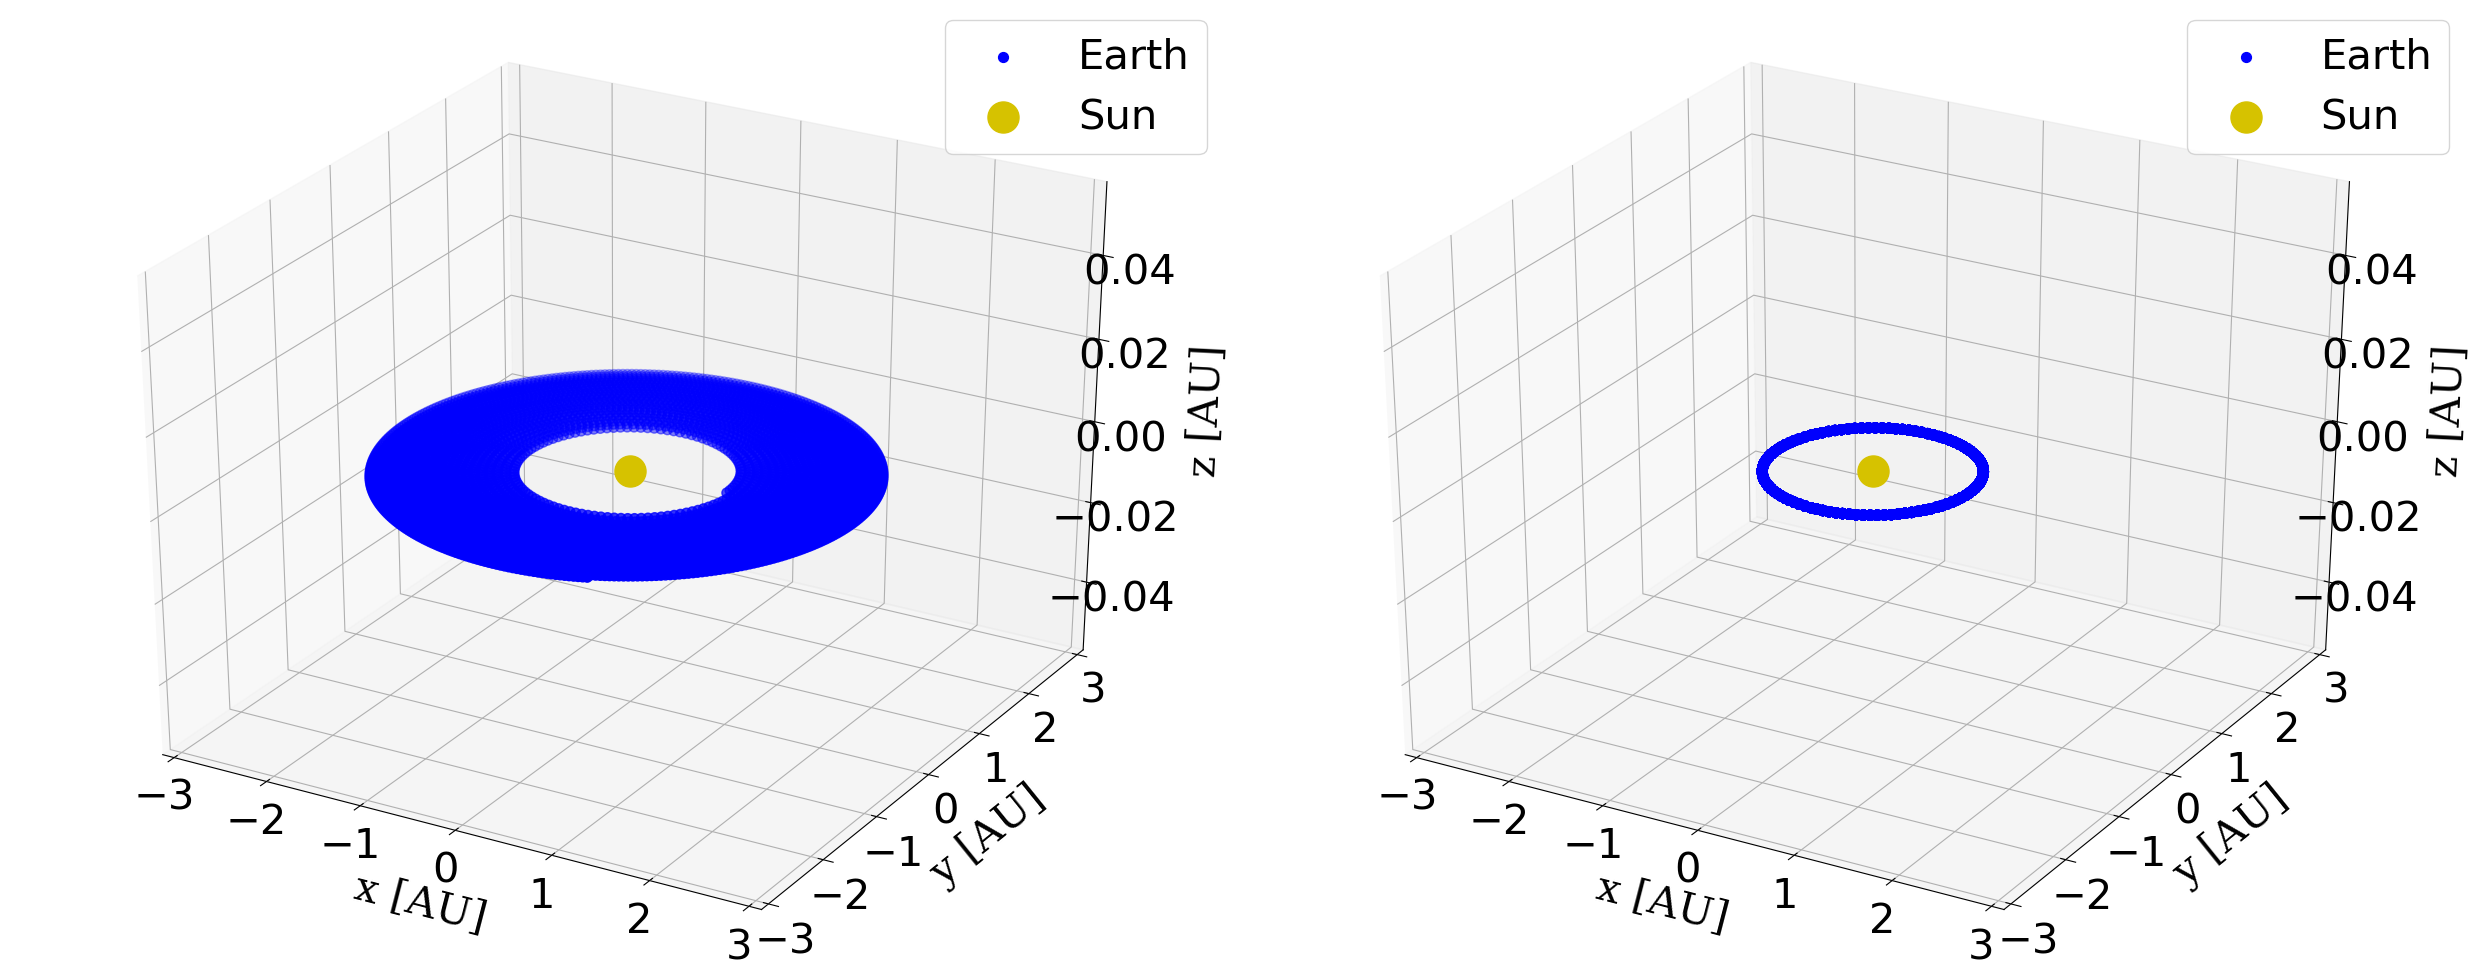
\includegraphics[keepaspectratio,height=10cm, width=12cm]{sun-earth-orbit.png}
  \caption{The trajectory of the Earth orbiting the Sun computed using the Forward Euler (left) and Velocity Verlet (right) methods. The trajectory is simulated for a period of $50$ years and we used a time step size of $0.001$ yr.}
   \label{euler_verlet_2body}
\end{figure}



To analyse the accuracy of the two numerical methods quantitatively, we computed the drift of the Earth's trajectory from a perfect circle. This can be achieved by computing the distance between the Sun and the Earth after the earth completes one orbit around the sun. Figure (\ref{euler_verlet_deviation1}) show the deviation of the trajectory from a circular orbit when computed using the Forward Euler and the Velocity Verlet methods as a function of the time step size. The error for both the Velocity Verlet and the Forward Euler method increases linearly in a loglog-scale with the time step. However, the error of the Velocity Verlet method is much smaller than that of the Forward Euler method.



For the Earth-Sun two-body problem with a circular orbit, we expect the kinetic energy, potential energy, total energy, and the angular momentum of the system to be conserved. Using the Forward Euler and the Velocity Verlet methods, we computed all these quantities as a function time. The deviation of the energies and angular momentum from their initial values are shown in figs. (\ref{Energy_Angmom_euler_verlet}) (left) and (right), respectively. As expected, the Velocity Verlet algorithm is energy and angular momentum conserving while the Forward Euler is not. Notice that the x- and y-component of the angular momentum are zero and hence we only show the z-component.
\begin{figure}[H]
  \centering
  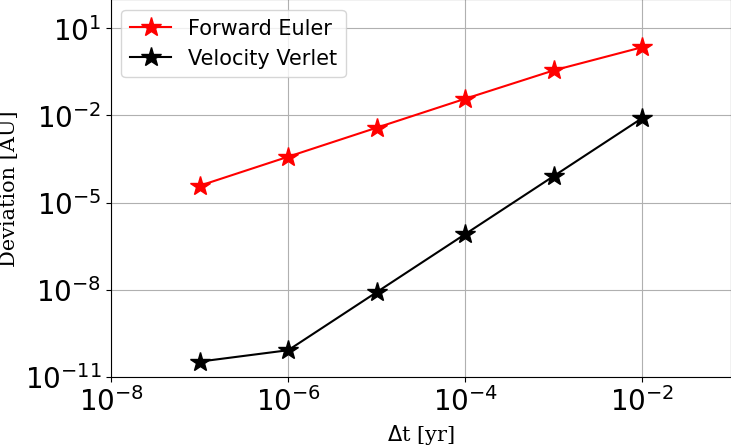
\includegraphics[keepaspectratio,height=10cm, width=10cm]{P03/Deviation_euler_verlet.png}
  \caption{The drift of the Earth's trajectory around the sun from a circular orbit as a function of the time step size when using the Velocity Verlet and the Forward Euler methods.}
   \label{euler_verlet_deviation1}
\end{figure}


\begin{figure}[H]
  \centering
  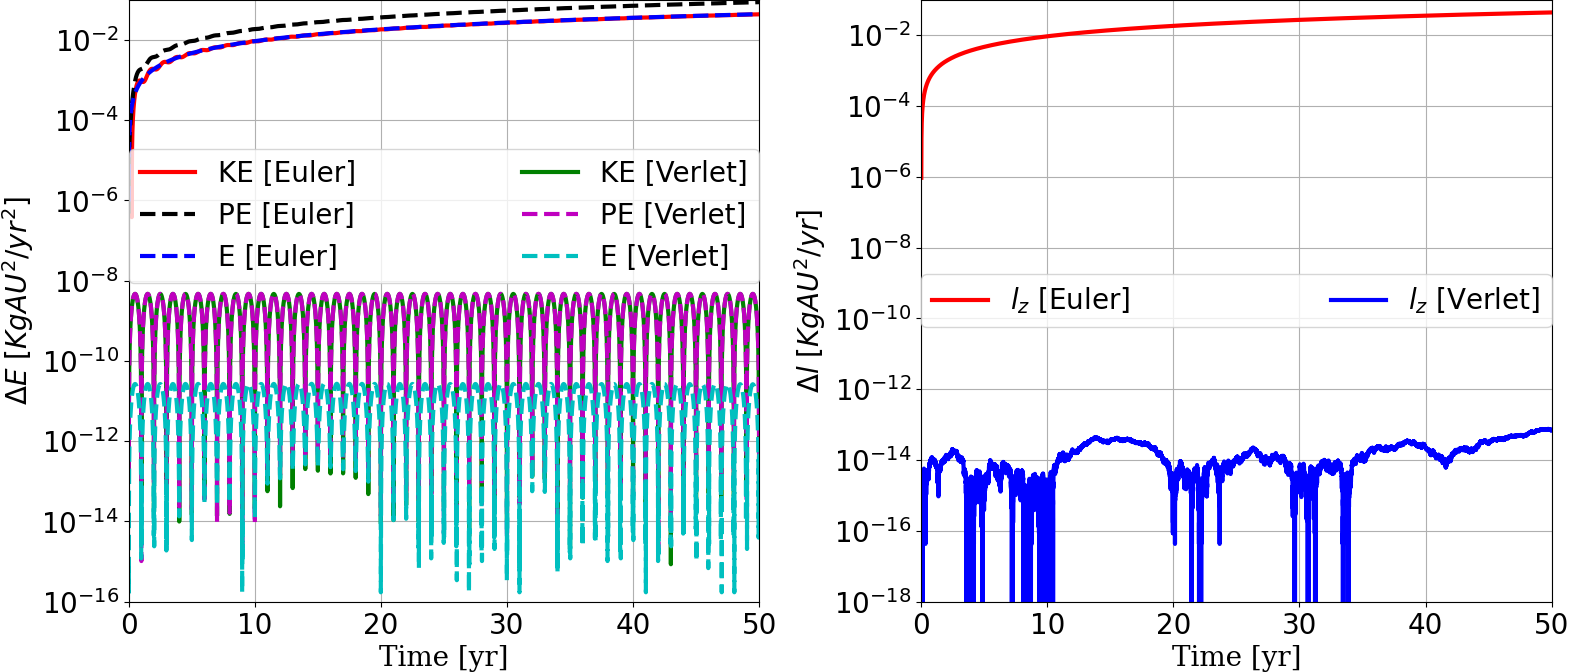
\includegraphics[keepaspectratio,height=10cm, width=12cm]{Energy_Angmom_euler_verlet_circle.png}
  \caption{The deviation of the energies (left) and the z-component of the angular momentum (right) from the initial values for the Earth-sun system as a function of time when using the Velocity Verlet and the Forward Euler methods. }
   \label{Energy_Angmom_euler_verlet}
\end{figure}

The CPU time consumption of the Forward Euler and the Velocity Verlet algorithms for solving the Earth-Sun two-body problem is shown in fig. (\ref{Time_euler_verlet}). The time consumption is computed by taking an average of running the algorithms $10$ times. For both the algorithms the time consumption increases linearly in a loglog-scale as the number of integration points increase. Moreover, we can see from fig. (\ref{Time_euler_verlet}) that the time consumption of the two algorithms is very similar, which is counter intuitive to our expectation based on the number of FLOPs.

\begin{figure}
  \centering
  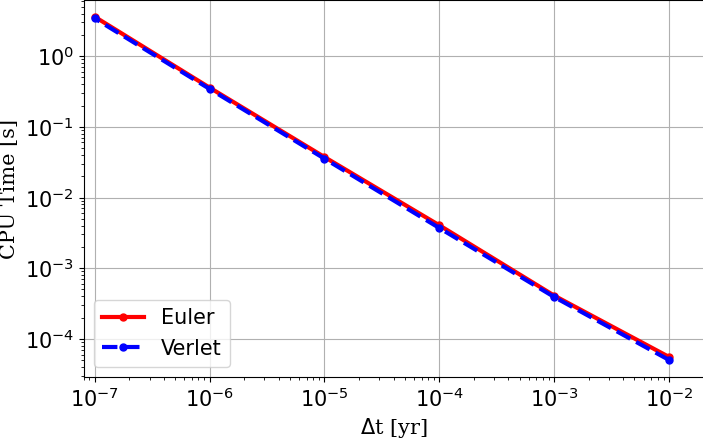
\includegraphics[keepaspectratio,height=10cm, width=8cm]{Time_euler_verlet.png}
  \caption{CPU time consumption as a function of the time step size for the Velocity Verlet and the Forward Euler methods. The maximum time for both methods is set to $1$ yr.}
   \label{Time_euler_verlet}
\end{figure}

Let us now investigate the consequences of having a gravitational law that is different from an inverse square relation. This is achieved by varying the exponent (denoted here by $\beta$) of the distance between the Earth and the Sun in Equation \ref{newton}. We considered a circular orbit for the Earth and varied the values of $\beta$ between $2$ and $3$ (cf. fig. (\ref{ModG_euler_verlet}) (left)). Using the Velocity Verlet algorithm with a very small time step size ($10^{-5}$ yr), all the values of $\beta$ we considered produced a stable circular orbit. This should not come as a surprise, because for a circular orbit with the radius fixed to $1$ AU, varying ${\beta}$ has no consequence for the trajectory. However, with a different radius or for an elliptical orbit it is only $\beta=2$ that can provide a stable orbit (cf. fig. (\ref{ModG_euler_verlet}) (right)). A slight change of the value to $\beta = 2.01$ resulted in an open elliptical orbit. When the value of $\beta$ is creeping towards $3$, Earth falls into the Sun and, as a consequence of instability in the Velocity Verlet algorithm, is ejected out off the solar system. 

\begin{figure}[H]
  \centering
  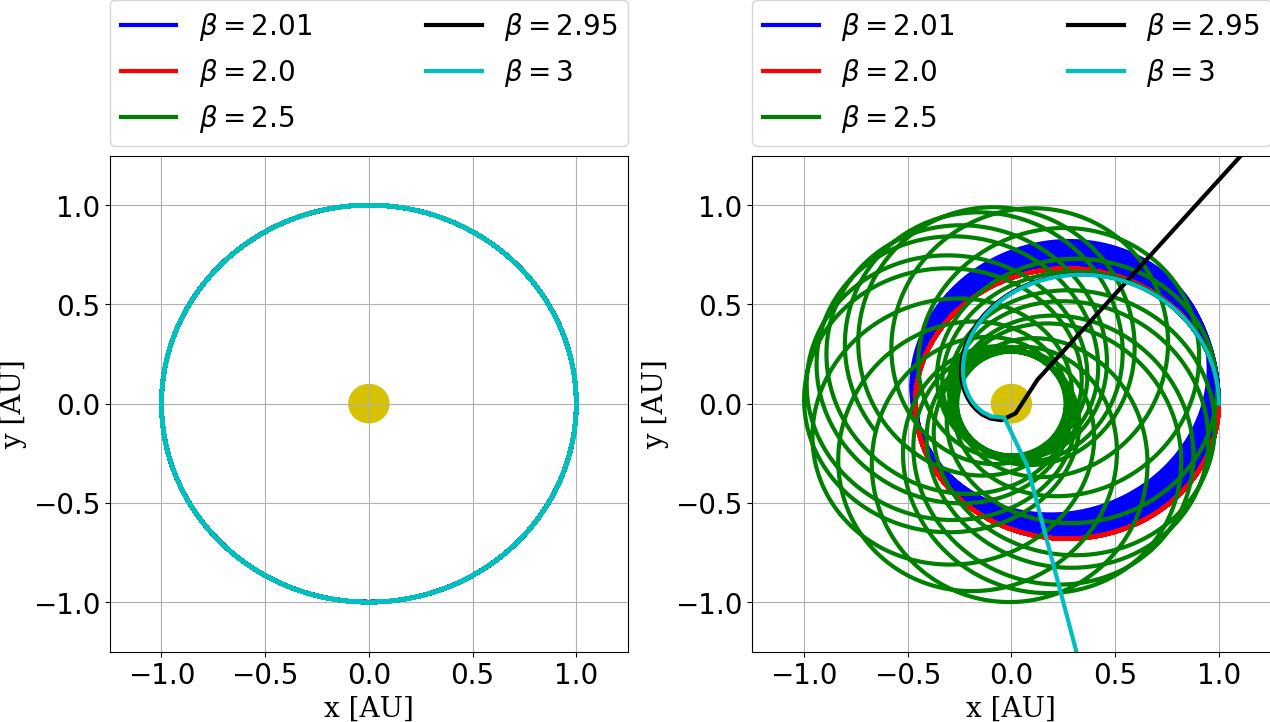
\includegraphics[keepaspectratio,height=12cm, width=12cm]{ModG_euler_verlet.png}
  \caption{The orbit of the Earth around the Sun as a consequence of different gravitational laws of the form $1/r^{\beta}$, with $\beta \in [2,3]$. The left plot is for the circular orbit while the right plot is for elliptical orbit.}
   \label{ModG_euler_verlet}
\end{figure}

Unlike for a circular orbit, the kinetic and potential energy of an elliptical orbit varies with time. However, the total energy and the angular momentum of the system are conserved for both circular and elliptical orbits (cf. fig. (\ref{Energy_Angmom_euler_verlet}) and (\ref{Energy_Angmom_verlet_ellipse})). For an elliptical orbit with gravitational force of $1/r^{3}$ dependence, the kinetic, potential, and the total energies are not conserved (cf. fig. (\ref{Energy_Angmom_verlet_ellipse_beta3}) (left)). However, the angular momentum of the system is still conserved for the gravitational force of $1/r^{3}$ dependence. This is due to the fact that for central forces the angular momentum of the system is always conserved.

\begin{figure}[H]
  \centering
  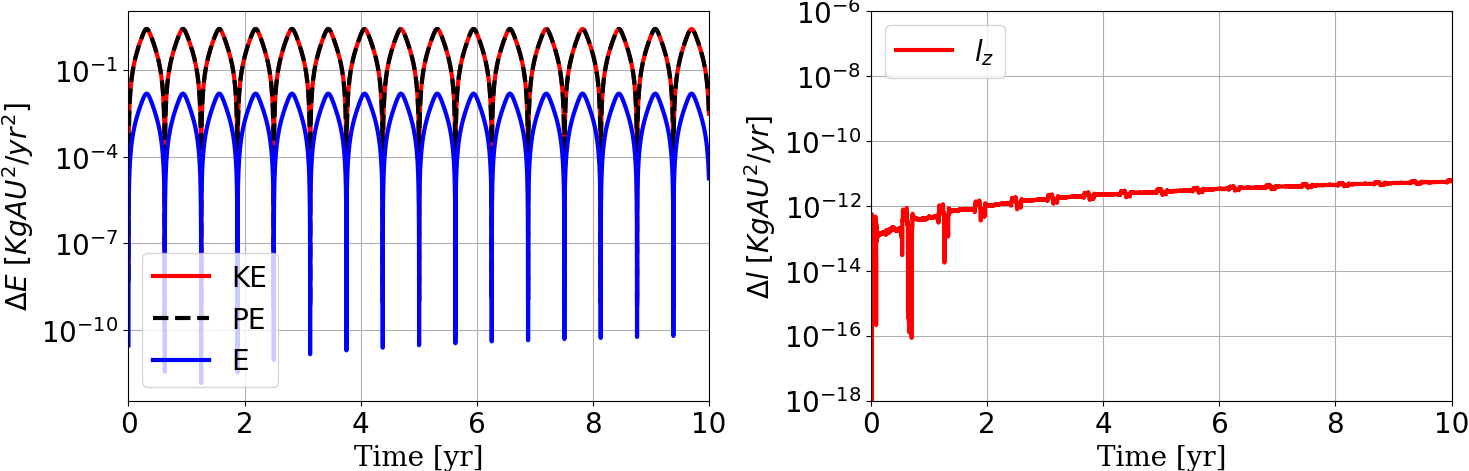
\includegraphics[keepaspectratio,height=10cm, width=12cm]{P03/Energy_Angmom_verlet_ellipse.png}
  \caption{The deviation from the initial values as a function of time of the energies (left) and the angular momentum (right) for an elliptical orbit of the Earth and an inverse square gravitation law. Here, we used the Velocity Verlet algorithm.}
   \label{Energy_Angmom_verlet_ellipse}
\end{figure}
\begin{figure}[H]
  \centering
  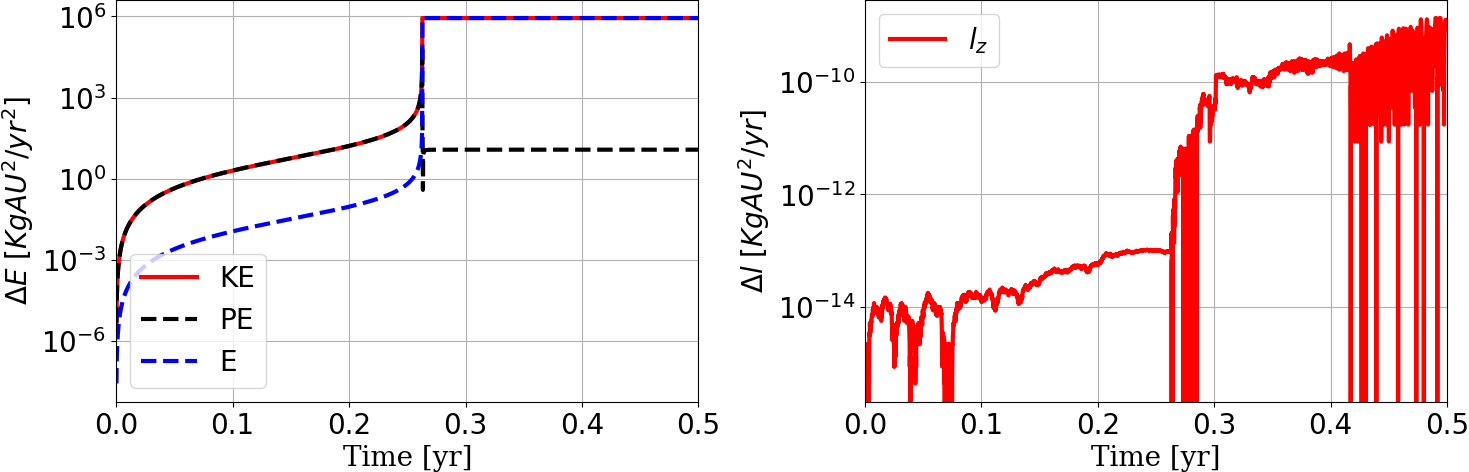
\includegraphics[keepaspectratio,height=10cm, width=12cm]{P03/Energy_Angmom_verlet_ellipse_beta3.png}
  \caption{The deviation from the initial values as a function of time of the energies (left) and the angular momentum (right)  for an elliptical orbit of the Earth and an inverse cubic gravitation law. Here, we used the Velocity Verlet algorithm. Notice the algorithm becomes unstable after $\sim 0.25$ yr.}
   \label{Energy_Angmom_verlet_ellipse_beta3}
\end{figure}

The velocity required for the Earth to escape the influence of the Sun's gravitational force is analytically derived in section \ref{escapeE} and it is equal to $2\pi\sqrt{2}$ AU/yr. To compute numerically this velocity we used the bisection method \cite{giordano} where we iteratively estimate and check if the Earth has escaped or not. We search for the escape velocity in a range between $2\pi$ and $4\pi$. Setting a maximum time of $1e3$ yr we estimated the escape velocity of the Earth to be $\sim 8.8848$ AU/yr. Comparing our numerical result with the analytical escape velocity, we notice our estimation has only $\sim 0.01\%$ relative error. 

Figure (\ref{Escape_Velocity}) show the trajectory of the Earth when the gravitational law is inverse square and cube. For the inverse square gravitation the trajectory of the Earth is shown with $99\%$ and at the escape velocity. For the inverse cube gravitation the trajectory of the Earth is shown at the corresponding escape velocity (i.e., $2\pi$ AU/yr). Notice, the difference in the trajectory for the two gravitation laws at their respective escape velocities.

\begin{figure}
  \centering
  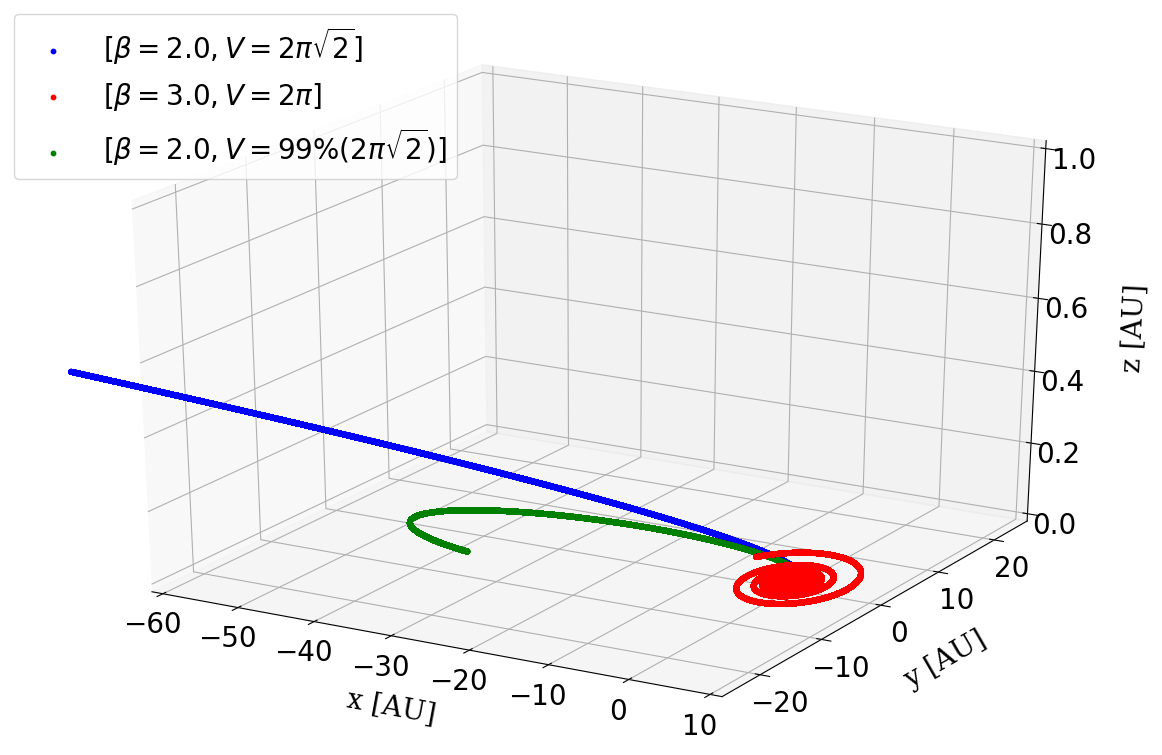
\includegraphics[keepaspectratio,height=10cm, width=12cm]{P03/Escape_Velocity.png}
  \caption{The trajectory of the Earth orbit around the Sun with initial velocities at $99 \%$ of the escape velocity and at the escape velocity. We show the orbits with inverse square and cube gravitational force.}
   \label{Escape_Velocity}
\end{figure}

\subsection{The Earth-Sun-Jupiter system}
We investigate the three-body problem consisting of the Sun, Earth, and Jupiter. First, we consider the Sun as stationary and located at the origin. The initial position and velocity for the Earth and Jupiter were extracted from the NASA webpage: \url{https://ssd.jpl.nasa.gov/horizons.cgi?s_loc=1#top}. The date and time corresponding to the initial conditions are: $A.D. 2020-Oct-09 00:00:00.0000$. We now consider three cases, (i) Jupiter with its actual mass, (ii) Jupiter with $10$ times its current mass, and (iii) Jupiter with $1000$ times its mass. For the first two cases the Earth and Jupiter have a closed and stable elliptical orbit. However, for the third case, the Earth first starts to orbit the Sun in a complex trajectory then moves and becomes the moon of Jupiter. All the computation is performed using a maximum time of $100$ yr and time step size of $10^{-5}$ yr (cf. fig. (\ref{Threebody})).

\begin{figure}
  \centering
  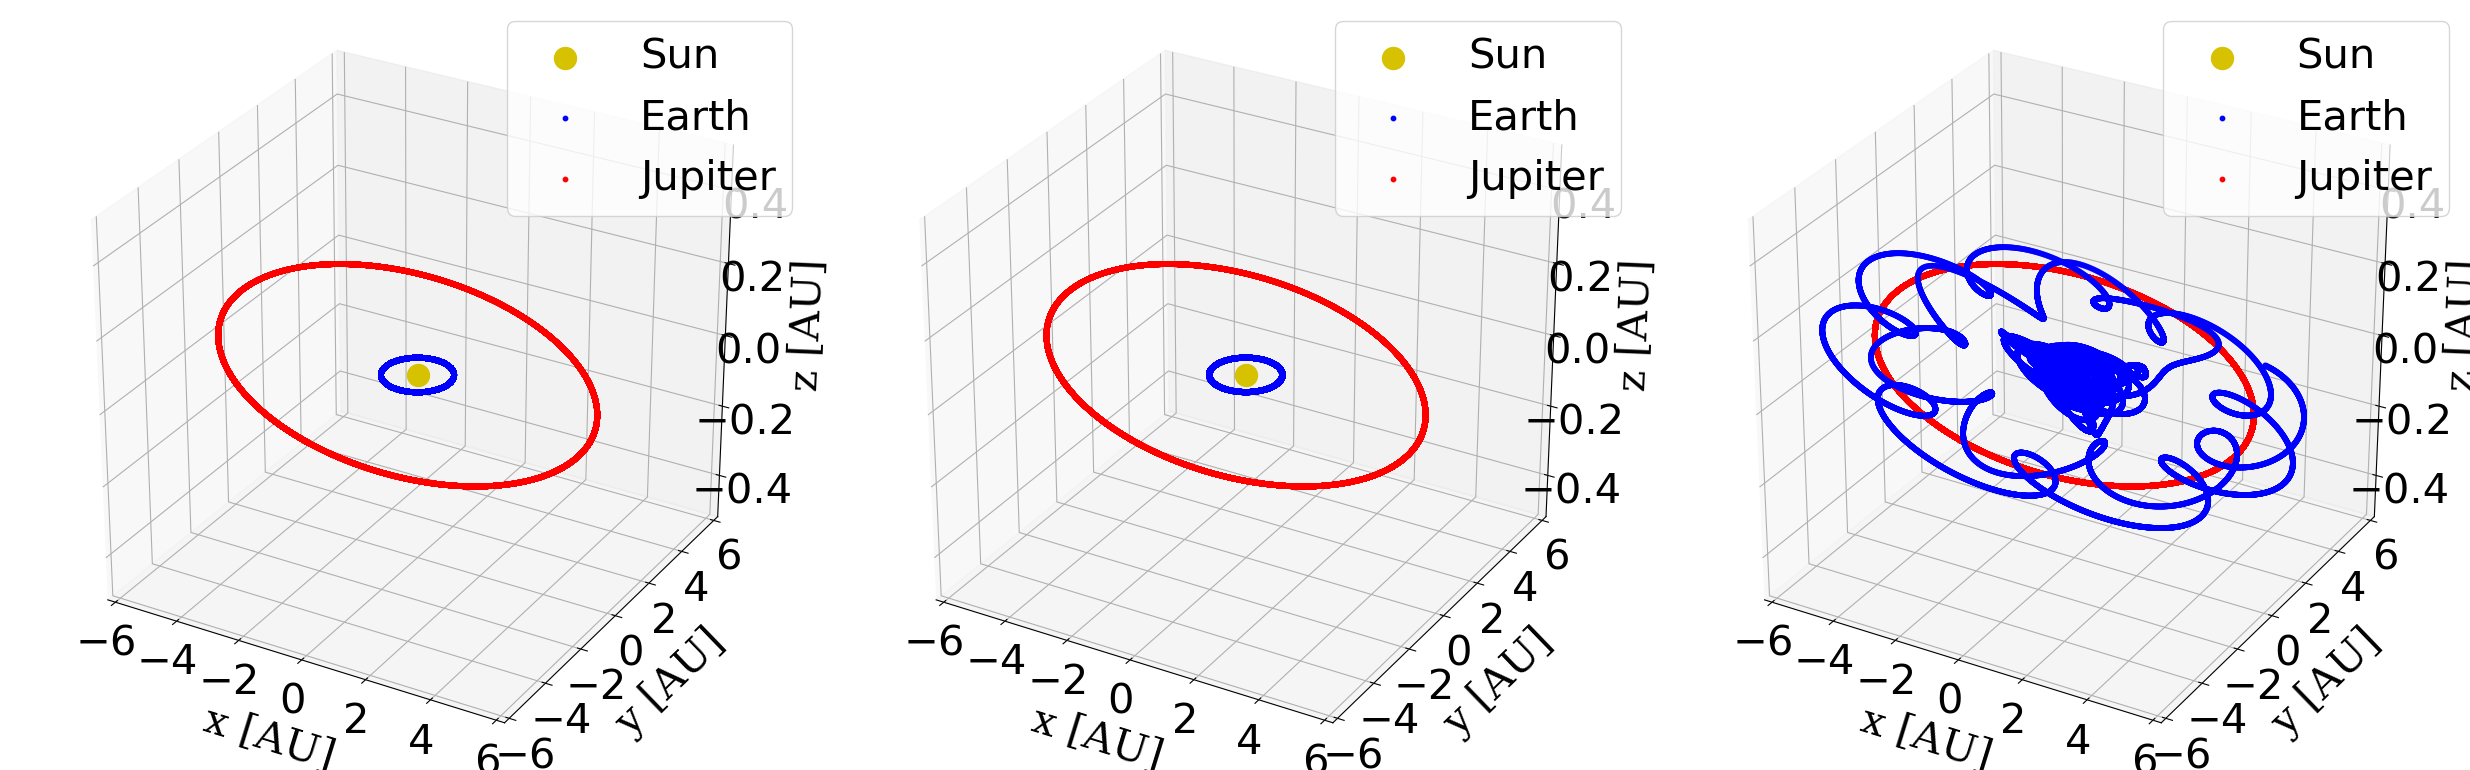
\includegraphics[keepaspectratio,height=10cm, width=12cm]{P03/Threebody.png}
  \caption{Simulation of the three-body problem with Sun-Earth-Jupiter and the Sun is fixed at the origin. Three scenarios are considered: Jupiter with its actual mass (left), $10$ times its mass (middle), and $1000$ times its mass. The simulation has a maximum time to $100$ yr and time step size of $10^{-5}$ yr.}
   \label{Threebody}
\end{figure}

We now allow the Sun to move and set the origin to its initial position. The initial velocity of the Sun is set so that the total momentum of the system is zero. Again, here we consider three masses for planet Jupiter. For the first two cases where the mass of Jupiter is $1$ and $10$ times its current mass, we observe that the trajectories of both Earth and Jupiter is elliptical, but for the latter case Earth slightly deviates from a stable orbit. However, when the mass of Jupiter is increased by a factor of $1000$ then the mass of Jupiter becomes comparable to that of the Sun. Consequently, the Sun and Jupiter form a binary star-configuration where they orbit each other, while the Earth keeps rotating around the Sun (cf. fig. (\ref{ThreebodyM})). 

\begin{figure}
  \centering
  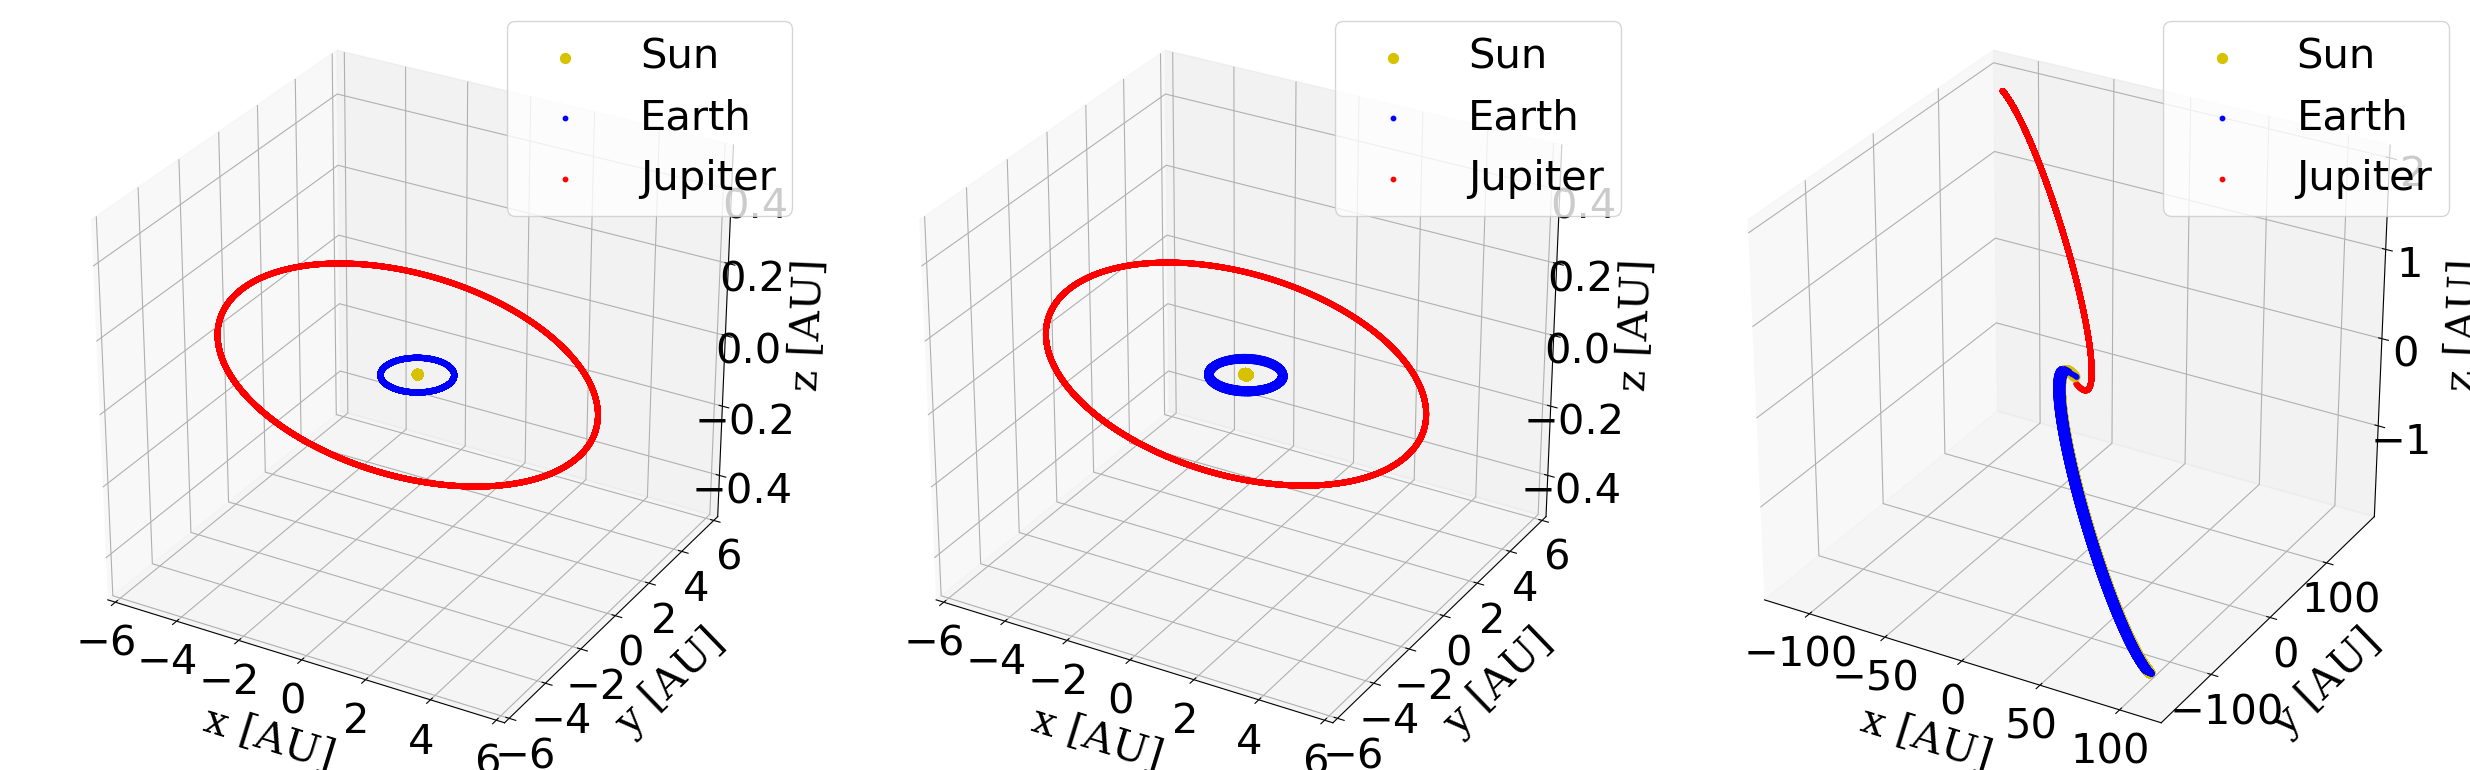
\includegraphics[keepaspectratio,height=10cm, width=12cm]{P03/ThreebodyM.png}
  \caption{Simulation of the three-body problem with Sun-Earth-Jupiter and the Sun is allowed to move. Three scenarios are considered: Jupiter with its actual mass (left), $10$ times its mass (middle), and $1000$ times its mass.The simulation has a maximum time to $1000$ yr and time step size of $10^{-5}$ yr.}
   \label{ThreebodyM}
\end{figure}

\subsection{The solar system}
The full solar system is a typical example of an $n$-body problem, where one of the masses (i.e., the Sun) is much larger than all the others. Nevertheless, in our simulation we account for the motion of the Sun and all the planets including the dwarf planet Pluto (cf. fig. (\ref{Full_solar_system})). Here, we use the Velocity Verlet algorithm with a time step size of $10^{-5}$ yr and all the initial conditions are obtained from NASA, except the initial velocity of the Sun which we set to a value that results in a zero total momentum for the system. All the trajectories of the planets appear stable, elliptical and in the same plane except that of Pluto, which has out-off plane orbit. \\

A live simulation of the full solar system is uploaded to the following github address: \url{https://github.com/endrias34/FYS4150/tree/master/doc/Project-3}.

\begin{figure}
  \centering
  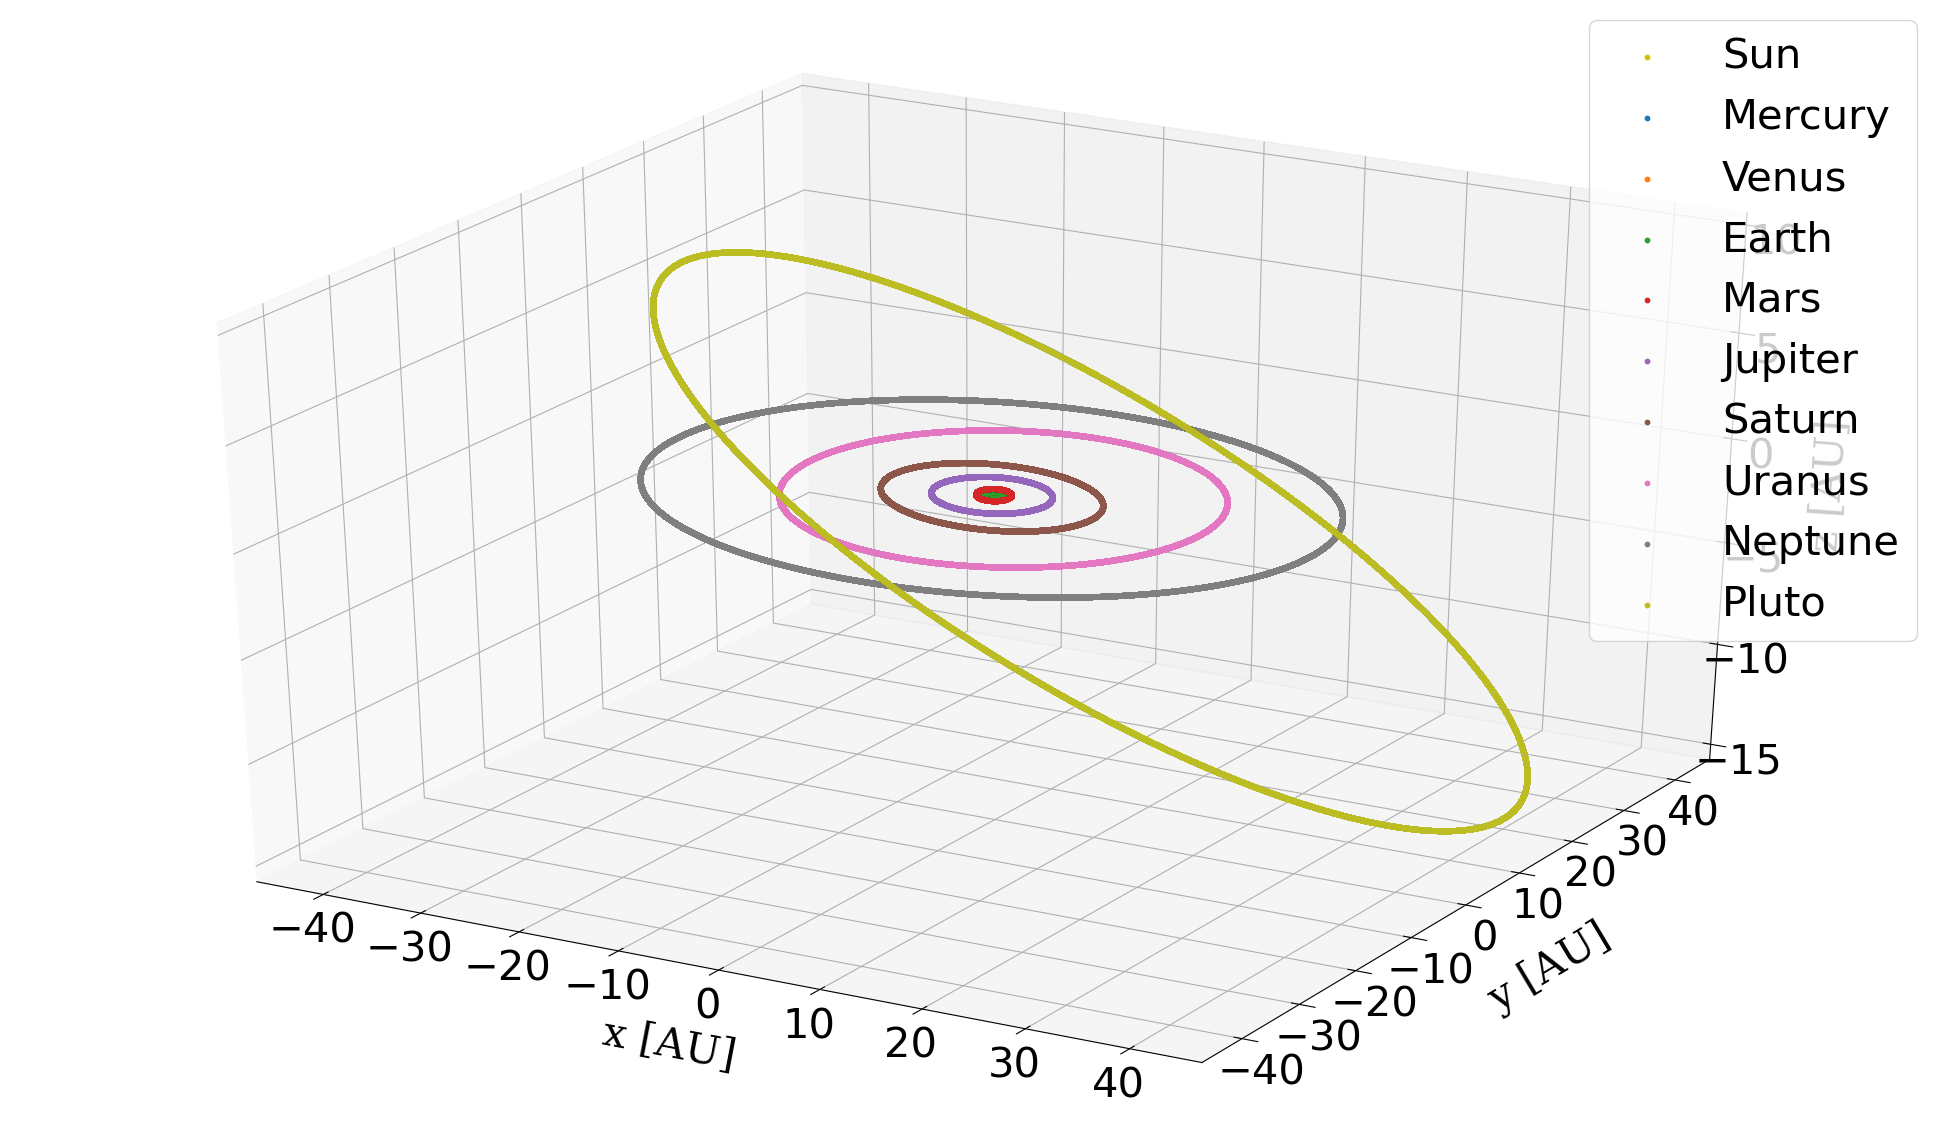
\includegraphics[keepaspectratio,height=10cm, width=12cm]{P03/Full_solar_system.png}
  \caption{Simulation of the full solar system with the addition of Pluto.}
   \label{Full_solar_system}
\end{figure}

\subsection{The perihelion precession of Mercury}
We computed the trajectory of the planet Mercury around the Sun for a period of a century using Newton's universal gravitation with and without relativistic corrections. For the initial speed and distance to the Sun at the perihelion, we have used $12.44$ AU/yr and $0.3075$ AU, respectively. Here, we have used the Velocity Verlet algorithm with a time step size of $10^{-7}$. After identifying the perihelion location after a century of orbit around the Sun, we calculated the perihelion angle. Consequently, we have found the perihelion angle of the orbit of the planet Mercury around the Sun when accounting and not accounting for the relativistic corrections are $42.9951$ and $0.243591$ arc seconds per century, respectively. The observed value for the perihelion precession of planet Mercury, when all classical effects are subtracted, is $43$ arc seconds per century. Therefore, our numerical computation including the relativistic correction produced the perihelion precession of planet Mercury with relative error of $0.01139\%$.

\section{Discussion}
Comparing the Forward Euler method with that of the Velocity Verlet method, we observed that the latter is more stable, has lower approximation error, and conserves both energy and angular momentum of the system. However, for a two-body problem with the Sun fixed at the center, we counted the number of FLOPs for the Forward Euler to be $27(N-1)$ while for the Velocity Verlet we have $57(N-1)$ FLOPs. Nevertheless, when computing the CPU time required by each algorithm, we observed a similar time for both algorithms. This counter intuitive observation might be caused by overheads in our code, which masks the actual time spent on the computations.

Kepler's laws are a direct consequence of the conservation of angular momentum and the fact that the gravitational force is an inverse square law \cite{giordano}. Moreover, Kepler's observational data show that the planets orbit elliptically around the Sun. To achieve such a stable orbit, our simulation suggested that the gravitational force needs to have precisely an inverse square relation. Nevertheless, we have also observed that for an inverse cubic gravitational force, the angular momentum is conserved. This is a consequence of the fact that the gravitational force is a central force, a force directed towards a fixed point in three dimensions and is spherically symmetric about that point \cite{goldstein}. Thus, for a central force the angular momentum is conserved. This explains why the angular momentum of a two-body problem is conserved for both the cases with the inverse square and inverse cubic gravitational force. 

To utilize observations, like that of Kepler's, to verify the inverse square law without accounting for the effects of the other bodies in the solar system is naive. Therefore, we have studied the effects of a three-body and a ten-body problem to investigate the trajectories of the different planets in our solar system. For the three-body problem containing the Sun, the Earth, and Jupiter, our simulation verified that the two planets orbit the Sun elliptically, except when we consider the case where planet Jupiter has $1000$ times its current mass. Such a case resulted in a binary stars system where the Earth is locked to orbiting the Sun. Here, we have also noticed that if the initial conditions (i.e., position and velocity) were different we would have gotten a completely different result. To simulate the full solar system, accounting for the motion of the Sun is very crucial. Although the Sun barely moves, accounting for its motion allows us to simulate as close as possible to the actual reality.

\section{Conclusion}
Coupled differential equations describing the dynamics of a two-, three-, and $n$-body problems were numerically solved using the Forward Euler and the Velocity Verlet algorithms.
The latter was found to be very stable, approximate better, and conserve both energy and angular momentum. For the two-body problem consisting of the Earth and the Sun, using the Velocity Verlet algorithm we were able to show that the Earth follows a stable elliptical trajectory only when the gravitational force is an inverse square law. Moreover, combining our simulation of the Earth-Sun system with the bisection method we found the escape velocity the Earth requires to overcome the Sun's gravitational pull is $\sim 8.8848$ AU/yr, which has only $\sim 0.01\%$ relative error compared to the exact analytical value ($2\sqrt{2}\pi$).

Simulating the Earth-Sun-Jupiter three-body problem with different hypothetical masses for planet Jupiter, we have seen that a stable result is only achieved only when considering a very small time step sizes (i.e., $< 10^{-5}$ yr). In addition, we have seen that the simulation is very sensitive to the initial conditions and it easily results in a chaotic trajectory, especially for the case with $1000$ times the current mass of Jupiter.

Finally, we simulated the full solar system and verified Kepler's first law where the different planets orbits the sun in a stable and elliptical orbit. Furthermore, we investigate the deviation of the gravitational force from the inverse square law by simulating the precession of the perihelion of planet Mercury. Accounting for the relativistic effects using the general theory of relativity, our simulation predicted the perihelion angle with a relative error of $0.01139\%$.

%\bibliographystyle{plain}
%\bibliographystyle{siam}
\bibliography{sample}
\bibliographystyle{IEEEtran}

\begin{appendix}
\section{Conservation of energy}
\label{app_eng}
Forward Euler method is not energy conserving. The proof provided here considers a physical system consisting of a block connected to a spring. This example is selected because of its simplicity for computing the acceleration, in this case it is given by -$\omega^2x$ \cite{Finite}. Thus, the position and velocity computed using the Forward Euler method is given by

\begin{align}
    \begin{bmatrix}
    x_{i+1} \\ v_{i+1} \\
  \end{bmatrix}
  =
    \begin{bmatrix}
        1 & h \\
        -\omega^2h & 1 
    \end{bmatrix}
    *
    \begin{bmatrix}
    x_i \\ v_i \\
  \end{bmatrix}.
\label{apdx-1}  
\end{align}


We see that the matrix in Equation \ref{apdx-1} has a determinant $(1 + \omega^2h^2)^{n}$, where n is the number of iterations. It is pertinent to notice that the determinant of a $2\times2$ matrix denotes the area spanned by the columns of the matrix.

\begin{figure}[H]
  \centering
  \includegraphics[keepaspectratio,height=10cm, width=12cm]{P03/area_determinant.png}
  \caption{Geometrical explanation of the determinant of a $2\times2$ matrix. Appeared in Mathematics Magazine, March 1985 \cite{determinant}.}
   \label{determinant}
\end{figure}

This means for a determinant other than $1$, we have an area spanned by the columns of our matrix that would shrink to zero or increase to infinity depending on our acceleration. Moreover, since the other terms in the matrix are fixed ($h$ and $1$), we have an acceleration function ($\omega$) that would spiral to zero or infinity, see fig. (\ref{euler_verlet_2body}) for the geometrical explanation. However, if we instead use our updated velocity for calculating the position we get the Euler Cromer method, which is energy conserving. We will not be using this method in this project, but for the interested reader a proof of the conservation is showed below. Again we use acceleration given by -$\omega^2x$ and thus the position and velocity updates becomes
\begin{equation}
v_{i+1} = v_{i} - \omega^2hx_{i}
\end{equation}
\begin{equation}
x_{i+1} = x_{i} + hv_{i+1}
\end{equation}
\begin{equation}
x_{i+1} = x_{i}(1 - \omega^2h^2) + hv_{i}
\end{equation}

Proof of conservation:

\begin{align}
    \begin{bmatrix}
    x_{i+1} \\ v_{i+1} \\
  \end{bmatrix}
  =
    \begin{bmatrix}
        1 - \omega^2h^2 & h \\
        - \omega^2h & 1 
    \end{bmatrix}
    *
    \begin{bmatrix}
    x_i \\ v_i \\
  \end{bmatrix}
\end{align}


det = $( (1 - \omega^2h^2) * 1 - h* (-\omega^2h))^{n} = 1^n$. We notice that the local error of the Euler-Cromer method is the same as the Forward Euler, $\epsilon = O(h^2)$. Finally, we provide a pseudo-code for the Euler-Cromer algorithm in Algorithm \ref{euler-cromer}.

\begin{algorithm}[H]
\caption{Euler-Cromer}
\textbf{Initial conditions:} $\mathbf{x_0}$ and $\mathbf{v_0}$ \\
\textbf{Input:} $h$
\begin{algorithmic}[1]
\While{$i\leq N$}
\For{\texttt{<each dimension>}}
\State $a_{i} = (-4\pi^2 * x_i) / r^3 $ \qquad// acceleration 
\State $v_{i+1}=v_{i} + h*a_{i}$ \qquad// Velocity
\State $x_{i+1}=x_{i} + h*v_{i+1}$ \qquad// Position
\EndFor
\EndWhile
\end{algorithmic}
\textbf{Output:} $\mathbf{x}$ and $\mathbf{v}$
\label{euler-cromer}
\end{algorithm}



\end{appendix}
\end{document}
